\documentclass[aspectratio=169]{ISAE-Beamer}
\usefonttheme[onlymath]{serif}
\usepackage{amsmath,amssymb,amsthm}
\usepackage{bm}
\usepackage{arydshln,mathtools}
\usepackage{graphicx}
\usepackage{diffcoeff}
\usepackage{dsfont}
\usepackage{mathrsfs}
\usepackage{tcolorbox}

%\usepackage{multimedia}
\usepackage{media9}
\usepackage[backend=bibtex]{biblatex}

\graphicspath{{../Figures/},{./Figures/}}

\bibliography{bib_pHMSD}

\DeclareMathOperator{\Tr}{Tr}
\DeclareMathOperator*{\grad}{grad}
\DeclareMathOperator*{\Grad}{Grad}
\DeclareMathOperator*{\Div}{Div}
\renewcommand{\div}{\operatorname{div}}
\DeclareMathOperator*{\Hess}{Hess}

\DeclareMathOperator*{\argmax}{arg\,max}
\DeclareMathOperator*{\argmin}{arg\,min}

\newcommand{\crmat}[1]{\ensuremath{[#1]_{\times}}}

\def\onedot{$\mathsurround0pt\ldotp$}
\def\cddot{% two dots stacked vertically
	\mathbin{\vcenter{\baselineskip.67ex
			\hbox{\onedot}\hbox{\onedot}}%
}}

\renewcommand\bibfont{\scriptsize}


\makeatletter \renewcommand\d[1]{\ensuremath{%
		\;\mathrm{d}#1\@ifnextchar\d{\!}{}}}
\makeatother

\title[INFIDHEM meeting]{Port-Hamiltonian flexible multibody dynamics}

\institute[ISAE]
{\inst{1}ISAE-SUPAERO, Toulouse}

\author[Andrea Brugnoli]{Andrea Brugnoli}

\date[Munich, 24/03/20]{Tuesday, the 24th, 2020}

%\thanks{}

\begin{document}

\maketitle

\begin{frame}{Outline}

\tableofcontents

\end{frame}

\section{Previous work on multibody systems and the pH formalism}

\begin{frame}{Previous wok}

Using Lie Algebra and differential forms a pH model of a flexible link has already been proposed \footfullcite{macchelli_fl}. This model can be embedded in a complex multibody system\footfullcite{macchelli_flrig}. \\
Advantages:
\begin{itemize}
	\item \onslide*<2->{Modular construction of flexible systems;}
	\item \onslide*<3->{Large deformations naturally considered.}
\end{itemize}
Disadvantages:
\begin{itemize}
	\item \onslide*<4->{Implementation really does not look trivial;}
	\item \onslide*<5->{Limited to one-dimensional systems;}
	\item \onslide*<6->{Numerical analysis not feasible;}
	\item \onslide*<7->{Model reduction techniques applicable.} 
\end{itemize}

\end{frame}

\section{Floating frame formulation of a floating body}

\begin{frame}{Floating frame based approach}
The floating frame approach relies on the hypothesis of small deformations: elastic motion is described w.r.t a reference that follows the large rigid motion. \\
Advantages
\begin{itemize}
	\item \onslide*<2->{The most used paradigm in multibody dynamics;}
	\item \onslide*<3->{For control applications most references adopt this approach;}
	\item \onslide*<4->{Model reduction techniques are applicable.} 
\end{itemize}
Disadvantages:
\begin{itemize}
	\item \onslide*<5->{Effect due to geometric non-linearities are not considered: not suitable for large deformation (substructuring can be employed to describe large deformations).}
\end{itemize}
\end{frame}

\begin{frame}{Floating body kinematics}
\onslide*<1>{
\begin{tcolorbox}
	\begin{figure}[t]
		\centering
		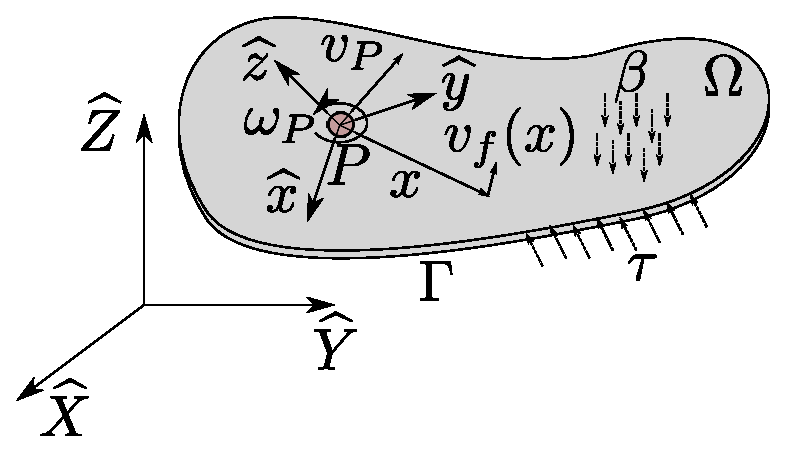
\includegraphics[width=0.6\textwidth]{floating_body.eps} 
		\caption{Thin floating body undergoing a surface traction $\bm\tau$ and body force density $\bm\beta$}
		\label{fig:float_body}
	\end{figure}
\end{tcolorbox}
}
\onslide*<2>{
The velocity of a generic point is expressed by considering a small flexible displacement superimposed to the rigid motion
\[
\bm{v} = \bm{v}_P + \crmat{\bm{\omega}_P} (\bm{x}+\bm{u}_f) + \bm{v}_f.
\]
This equation is expressed in the body reference frame $\widehat{\bm{x}}, \widehat{\bm{y}}, \widehat{\bm{z}}$.  
\begin{itemize}
	\item $\bm{x}$ is the position vector of the current point;
	\item $\bm{v}_P,\, \bm{\omega}_P$ are the linear and angular velocities of point $P$;
	\item $\bm{v}_f := \dot{\bm{u}}_f$ is the time derivative of the deformation displacement $\bm{u}_f$ (computed in the body frame); 
	\item The cross map $\crmat{\bm{a}}$ denotes the skew-symmetric matrix associated to vector $\bm{a}$.
\end{itemize}

}
\end{frame}

\begin{frame}{Equations of motion}
The equations are obtained by application of the virtual work principle \footfullcite[Chapter 4]{simeon2013computational}. \\
\begin{overlayarea}{\textwidth}{0.8\textheight}
\only<1-2> {
	\only<1>{ Linear momentum balance:
	\begin{equation*}
	\begin{split}
	&m (\dot{\bm{v}}_P + \crmat{\bm{\omega}_P} \bm{v}_P) + \crmat{\bm{s}_u}^\top \dot{\bm{\omega}}_P  + \int_{\Omega} \rho \ddot{\bm{u}}_f \d{\Omega} = \\
	&\quad - \crmat{\bm{\omega}_P} \crmat{\bm{\omega}_P} \bm{s}_u - \int_{\Omega} 2 \rho \crmat{\bm{\omega}_P} \dot{\bm{u}}_f \d{\Omega} +  \int_{\Omega} \bm\beta \d{\Omega} + \int_{\partial \Omega} \bm\tau \d{\Gamma},
	\end{split}
	\end{equation*}
}
\only<2>{
	Rearranged linear momentum balance:
	\begin{equation*}
	\begin{split}
	m\dot{\bm{v}}_P + \crmat{\bm{s}_u}^\top \dot{\bm{\omega}}_P +   \int_{\Omega} \rho \dot{\bm{v}}_f \d{\Omega}  = \\
	\left[m \bm{v}_P + \crmat{\bm{s}_u}^\top \bm\omega_P +2 \int_{\Omega} \rho \bm{v}_f \d{\Omega} \right]_\times \bm\omega_P +  \int_{\Omega} \bm\beta \d{\Omega} + \int_{\partial \Omega} \bm\tau \d{\Gamma}.
	\end{split}
	\end{equation*}
}
	\begin{itemize}
		\item $\rho$ is the mass density;
		\item $m = \int_{\Omega} \rho \d{\Omega}$ the total mass;
		\item  $\bm{s}_u = \int_{\Omega} \rho (\bm{x}+\bm{u}_f) \d{\Omega}$ the static moment.
	\end{itemize}
	}

\only<3-4> {
	\only<3>{Angular momentum balance:
	\begin{equation*}
	\begin{split}
	\crmat{\bm{s}_u} (\dot{\bm{v}}_P + \crmat{\bm{\omega}_P} \bm{v}_P) + \bm{J}_u \dot{\bm\omega}_P + \int_{\Omega} \rho \crmat{\bm{x}+\bm{u}_f} \ddot{\bm{u}}_f \d{\Omega} + \crmat{\bm{\omega}_P} \bm{J}_u \bm{\omega}_P = \\ 
	- \int_{\Omega} 2\rho \crmat{\bm{x}+\bm{u}_f} \crmat{\bm\omega_P} \dot{\bm{u}}_f \d{\Omega} + \int_{\Omega}\crmat{\bm{x}+\bm{u}_f} \bm\beta \d{\Omega} + \int_{\partial \Omega}\crmat{\bm{x}+\bm{u}_f} \bm\tau \d{\Gamma}, \\
	\end{split}
	\end{equation*}
	}
\only<4>{Rearranged angular momentum balance:
	\begin{equation*}
	\begin{split}
	\crmat{\bm{s}_u} \dot{\bm{v}}_P  + \bm{J}_u \dot{\bm\omega}_P + \int_{\Omega} \rho \crmat{\bm{x}+\bm{u}_f} \dot{\bm{v}}_f \d{\Omega} = \\
	\left[\crmat{\bm{s}_u}^\top \bm\omega_P + 2 \int_{\Omega} \rho \bm{v}_f \d{\Omega} \right]_\times \bm{v}_P + \left[\crmat{\bm{s}_u} \bm{v}_P + \bm{J}_u \bm\omega_P + 2 \int_{\Omega} \rho \crmat{\bm{x}+\bm{u}_f} {\bm{v}}_f \d{\Omega} \right]_\times \bm\omega_P + 
	\\
	2 \int_{\Omega} \left[\rho \bm{v}_P + \rho \crmat{\bm{x}+\bm{u}_f}^\top \, \bm\omega_P \right]_\times \bm{v}_f \d{\Omega} + \int_{\Omega}\crmat{\bm{x}+\bm{u}_f} \bm\beta \d{\Omega} + \int_{\partial \Omega}\crmat{\bm{x}+\bm{u}_f} \bm{\tau} \d{\Gamma}.
	\end{split}
	\end{equation*}}
\vspace{2cm}
$\bm{J}_u:= \int_{\Omega} \rho \crmat{\bm{x}+\bm{u}_f}^\top\crmat{\bm{x}+\bm{u}_f} \d{\Omega}$ is the inertia matrix.
}
\only<5-6> {\only<5>{Flexibility PDE:
	\begin{equation*}
	\begin{split}
	\rho (\dot{\bm{v}}_P + \crmat{\bm\omega_P} \bm{v}_P) + \rho (\crmat{\dot{\bm\omega}_P} + \crmat{\bm{\omega}_P}\crmat{\bm{\omega}_P})(\bm{x}+\bm{u}_f) + \rho (2 \crmat{\bm{\omega}_P} \dot{\bm{u}}_f + \ddot{\bm{u}}_f) = \\
	\Div{\bm\Sigma} + \bm\beta,
	\end{split}
	\end{equation*}}
	\only<6>{Rearranged llexibility PDE:
		\begin{equation*}
		\begin{split}
		\rho \dot{\bm{v}}_P + \rho \crmat{\bm{x}+\bm{u}_f}^\top \dot{\bm\omega}_P  + \rho \dot{\bm{v}}_f = \\
		\left[\rho \bm{v}_P + \rho \crmat{\bm{x}+\bm{u}_f}^\top \bm\omega_P + 2 \rho \bm{v}_f \right]_\times \bm\omega_P + \Div{\bm\Sigma} + \bm\beta.
		\end{split}
		\end{equation*}
	}
	together with boundary conditions
	\begin{equation*}
	\begin{aligned}
	&\text{Neumann condition} \\
	&\text{Dirichlet condition} \\
	\end{aligned} \quad
	\begin{aligned}
	\bm\Sigma \cdot \bm{n}|_{\Gamma_N} &= \bm\tau|_{\Gamma_N}, \quad \text{$\bm{n}$ is the outward normal,} \\
	\bm{u}_f|_{\Gamma_D} &= \bm{\bar{u}}_f|_{\Gamma_D},
	\end{aligned}
	\end{equation*}
	\begin{itemize}
		\item $\bm\Sigma$ is the Cauchy stress tensor;
		\item The infinitesimal strain is given by $\bm\varepsilon  =  \Grad(\bm{u}_f) \quad \Grad = \frac{1}{2}[\nabla+\nabla^\top]$;
		\item To close the system,  Hooke's law $\bm\Sigma =  \bm{\mathcal{D}} \bm\varepsilon$, where $ \bm{\mathcal{D}}$ is the stiffness tensor.
	\end{itemize}
	}
\end{overlayarea}
\end{frame}


\section{A pH formation of floating bodies}

\begin{frame}{Energies and canonical momenta}
\begin{overlayarea}{\textwidth}{0.95\textheight}
Consider the total energy (Hamiltonian), given by the sum of kinetic and deformation energy:
\begin{equation*}
\label{eq:H}
\begin{aligned}
H &= H_{\text{kin}} + H_{\text{def}}, \\
&= \frac{1}{2} \int_{\Omega} \left\{\rho ||\bm{v}_P + \crmat{\bm{\omega}_P} (\bm{x}+\bm{u}_f) + {\bm{v}}_f||^2 + \bm\Sigma \cddot \bm\varepsilon \right\}  \d{\Omega}.
\end{aligned}
\end{equation*}

\only<1>{ The momenta (usually called energy variables in the pH framework) are then computed by derivation of the Hamiltonian: 
\begin{equation*}
\label{eq:momenta}
\begin{aligned}
\bm{p}_t &:= \diffp{H}{\bm{v}_P} = m \bm{v}_P + \crmat{\bm{s}_u}^\top \, \bm\omega_P + \int_{\Omega} \rho \bm{v}_f \d{\Omega}, \\
\bm{p}_r &:= \diffp{H}{\bm\omega_P} = \crmat{\bm{s}_u} \bm{v}_P + \bm{J}_u \bm\omega_P + \int_{\Omega} \rho \crmat{\bm{x}+\bm{u}_f} \bm{v}_f \d{\Omega}, \\
\bm{p}_f &:= \diffd{H}{\bm{v}_f} = \rho \bm{v}_P + \rho \crmat{\bm{x}+\bm{u}_f}^\top \, \bm\omega_P + \rho \bm{v}_f, \\
\bm\varepsilon &:= \diffd{H}{\bm\Sigma} = \bm{\mathcal{D}}^{-1} \bm\Sigma,
\end{aligned}
\end{equation*}
}
\only<2>{In matrix form
	\begin{equation*}
	\begin{bmatrix}
	\bm{p}_t \\ \bm{p}_r \\ \bm{p}_f \\ \bm\varepsilon \\
	\end{bmatrix} = 
	\underbrace{\begin{bmatrix}
		m \bm{I}_{3\times 3} & \crmat{\bm{s}_u}^\top & \mathcal{I}_\rho^{\Omega} & 0 \\
		\crmat{\bm{s}_u} & \bm{J}_u & \bm{\mathcal{I}}_{\rho x}^{\Omega} & 0  \\
		(\mathcal{I}_\rho^{\Omega})^* & (\bm{\mathcal{I}}_{\rho x}^{\Omega})^* & \rho & 0  \\
		0 & 0 & 0 & \bm{\mathcal{D}}^{-1} \\
		\end{bmatrix}}_{\bm{\mathcal{M}}: \; \text{Mass operator}}
	\begin{bmatrix}
	\bm{v}_P \\ \bm{\omega}_P  \\ \bm{v}_f  \\ \bm\Sigma \\
	\end{bmatrix}, \qquad 
	\begin{aligned}
	\mathcal{I}_\rho^\Omega &:=\int_{\Omega} \rho (\cdot) \d{\Omega}, \\
	\bm{\mathcal{I}}_{\rho x}^{\Omega} &:= \int_\Omega \rho \crmat{\bm{x}+\bm{u}_f} (\cdot). \\
	\end{aligned}
	\end{equation*}	
	
}
\only<3>{The mass operator $\bm{\mathcal{M}}$ is a self-adjoint, positive operator. It holds
\begin{equation*}
H_{\text{kin}} + H_{\text{def}} = \frac{1}{2} \langle \bm{e}_{\text{kd}}, \ \bm{\mathcal{M}} \bm{e}_{\text{kd}} \rangle, \qquad \bm{e}_{\text{kd}} = [\bm{v}_P; \, \bm{\omega}_P; \, \bm{v}_f; \bm{\Sigma}]
\end{equation*}
Notice that the kinetic energy also depends on the flexible displacement
\[
\diffd{H_{\text{kin}}}{\bm{u}_f} = \crmat{\bm{p}_f} \bm{\omega_{P}}.
\]
This term is responsible for a coupling between the kinematic coordinates and the velocities.
}
\end{overlayarea}
\end{frame}

\begin{frame}{PH formulation}
\only<1>{Generalized coordinates are required for a complete formulation:
\begin{itemize}
	\item $^i \bm{r}_P$ the position of point $P$ in the inertial frame of reference;
	\item $\bm{R}$ the direction cosine matrix that transforms vectors from the body frame to the inertial frame (other attitude parametrizations are possible);
	\item $\bm{u}_f$ the flexible displacement;
\end{itemize}
The direction cosine matrix is converted into a vector by concatenating its rows
\begin{equation*}
\bm{R}_{\text{v}} = \text{vec}(\bm{R}^\top) = [\bm{R}_x \; \bm{R}_y \; \bm{R}_z]^\top,
\end{equation*}
where $\bm{R}_{x}, \bm{R}_{y}, \bm{R}_{z}$ are the first, second and third row of matrix $\bm{R}$. Furthermore the corresponding cross map will be given by
\begin{equation*}
\crmat{\bm{R}_{\text{v}}} = 
\begin{bmatrix}
\crmat{\bm{R}_x} \\
\crmat{\bm{R}_y} \\
\crmat{\bm{R}_z} \\
\end{bmatrix}, \qquad 
\crmat{\bm{R}_{\text{v}}} : \mathbb{R}^9 \rightarrow \mathbb{R}^{9 \times 3}.
\end{equation*}
}
\only<2>{ The overall port-Hamiltonian formulation
\begin{equation*}
\setlength{\dashlinegap}{2pt}
\underbrace{
	{\left[ \begin{array}{c:c}
		\bm{I} & 0 \\
		\hdashline
		0 & \bm{\mathcal{M}} \\
		\end{array} \right]}
}_{\bm{\mathcal{E}}}
\diff{}{t}
\underbrace{\begin{bmatrix}
	^i \mathbf{r}_P \\ \bm{R}_{\text{v}} \\ \bm{u}_f \\\hdashline  \bm{v}_P \\ \bm\omega_P  \\ \bm{v}_f  \\ \bm\Sigma \\
	\end{bmatrix}}_{\bm{e}} = 
\underbrace{
	{\left[ \begin{array}{ccc:cccc}
		0 & 0 & 0 &  \bm{R} & 0 & 0 & 0 \\
		0 & 0 & 0 & 0 & \crmat{\bm{R}_{\text{v}}} & 0 & 0 \\
		0 & 0 & 0 & 0 & 0 & \bm{I}_{3\times 3} & 0  \\ 
		\hdashline
		-\bm{R}^\top & 0 & 0 & 0 & \crmat{\widetilde{\bm{p}}_t} & 0 & 0 \\
		0 & -\crmat{\bm{R}_{\text{v}}}^\top & 0 & \crmat{\widetilde{\bm{p}}_t} & \crmat{\widetilde{\bm{p}}_r} & \bm{\mathcal{I}}_{p_f}^\Omega & 0 \\
		0 & 0 & -\bm{I}_{3\times 3} & 0 & -(\bm{\mathcal{I}}_{p_f}^\Omega)^* & 0 & \Div \\
		0 & 0 & 0 & 0 & 0 & \Grad & 0 \\
		\end{array} \right]}
}_{\bm{\mathcal{J}}}
\underbrace{\begin{bmatrix}
	\partial_{\bm{r}_P}H \\ \partial_{\bm{R}_\text{v}}H \\ \delta_{\bm{u}_f} H \\\hdashline  \bm{v}_P \\ \bm\omega_P  \\ \bm{v}_f  \\ \bm\Sigma \\
	\end{bmatrix}}_{\bm{z}}.
\end{equation*} 
Variables $\widetilde{\bm{p}}_t, \widetilde{\bm{p}}_r$ are defined as: 
\[\widetilde{\bm{p}}_t = \bm{p}_t + \int_{\Omega} \rho \bm{v}_f \d{\Omega}, \qquad \widetilde{\bm{p}}_r = \bm{p}_r + \int_{\Omega} \rho \crmat{\bm{x} + \bm{u}_f}\bm{v}_f \d{\Omega}.\]
The operator $\bm{\mathcal{I}}_{p_f}^\Omega$ is defined as: $\bm{\mathcal{I}}_{p_f}^\Omega := \int_\Omega \left\{2 \crmat{\bm{p}_f} + \rho \crmat{\bm{v}_f} \right\}(\cdot) \d{\Omega}$.
}
\end{frame}

\begin{frame}{Floating body as a pHDAE system}
This system fits into the framework detailed in \footfullcite{mehrmann2019structurepreserving} and extends it.
\begin{equation*}
\begin{aligned}
\bm{\mathcal{E}}(\bm{e}) \diffp{\bm{e}}{t} &= \bm{\mathcal{J}}(\bm{e}) \bm{z}(\bm{e}) + \bm{\mathcal{B}}_d(\bm{e}) \bm{u}_d + \bm{\mathcal{B}}_r(\bm{e}) \bm{u}_\partial, \qquad \text{where } \bm{u}_d:=\bm\beta \\
\bm{y}_d &= \bm{\mathcal{B}}_d^*(\bm{e}) \bm{z}(\bm{e}), \\
\bm{y}_r &= \bm{\mathcal{B}}_r^*(\bm{e}) \bm{z}(\bm{e}), \\
\bm{u}_\partial &= \bm{\mathcal{B}}_{\partial} \bm{z}(\bm{e}) =  \bm\Sigma \cdot \bm{n}|_{\partial \Omega} = \bm\tau|_{\partial \Omega}, \\
\bm{y}_\partial &= \bm{\mathcal{C}}_{\partial} \bm{z}(\bm{e}) = \bm{v}_f|_{\partial \Omega},
\end{aligned}
\end{equation*}
Vector $\bm{y}_r$ represents the rigid body velocity at the boundary $\bm{y}_r = (\bm{v}_P + \crmat{\bm{x}+\bm{u}_f}^\top \bm{\omega}_P)\vert_{\partial\Omega}$, \\
while $\bm{y}_d$ represents the velocity field in the domain $\bm{y}_d = (\bm{v}_P + \crmat{\bm{x}+\bm{u}_f}^\top \bm{\omega}_P + \bm{v}_f)\vert_{\Omega}$.
Operator $\bm{\mathcal{E}}$ is positive self-adjoint, $\bm{\mathcal{J}}$ is formally skew-symmetric.
The Hamiltonian  satisfies 
\begin{equation*}
\partial_{\bm{e}} H = \bm{\mathcal{E}}^* \bm{z}.
\end{equation*}

\end{frame}

\begin{frame}{Energy balance}
\begin{equation}
\begin{aligned}
\dot{H}(\bm{e}) &= \langle \partial_{\bm{e}} H, \partial_t {\bm{e}} \rangle_{\mathscr{X}} = \langle \bm{\mathcal{E}}^* \bm{z}, \partial_t {\bm{e}} \rangle_{\mathscr{X}}, \\
&= \langle \bm{z}, \bm{\mathcal{E}} \partial_t {\bm{e}} \rangle_{\mathscr{X}}, \quad \text{Adjoint definition}, \\
& = \langle \bm{z}, \bm{\mathcal{J}}\bm{z} + \bm{\mathcal{B}}_d(\bm{e}) \bm{u}_d + \bm{\mathcal{B}}_r(\bm{e}) \bm{u}_\partial \rangle_{\mathscr{X}}, \\
& = \langle \bm{y}_\partial,  \bm{u}_\partial \rangle_{\mathscr{L}^2(\partial\Omega, \mathbb{R}^3)} + \langle \bm{\mathcal{B}}_d^* \bm{z}, \bm{u}_d \rangle_{\mathscr{X}} + \langle \bm{\mathcal{B}}_r^* \bm{z}, \bm{u}_\partial \rangle_{\mathscr{X}}, \quad \text{I.B.P. on } \bm{\mathcal{J}}, \\
&= \langle \bm{y}_\partial + \bm{y}_r,  \bm{u}_\partial \rangle_{\mathscr{L}^2(\partial\Omega, \mathbb{R}^3)} + \langle \bm{y}_d,  \bm{u}_d \rangle_{\mathscr{L}^2(\Omega, \mathbb{R}^3)}, \\
\end{aligned}
\end{equation}
where the integration by parts (Stokes theorem) has been used
\begin{equation}
\label{eq:stokes}
\int_{\Omega} \bm\Sigma \cddot \Grad(\bm{v}_f) \d{\Omega} + \int_{\Omega} \Div(\bm\Sigma) \cdot \bm{v}_f \d{\Omega} = \int_{\partial \Omega} (\bm\Sigma \cdot \bm{n}) \cdot \bm{v}_f \d{\Gamma} = \langle \bm{y}_\partial,  \bm{u}_\partial \rangle_{\mathscr{L}^2(\partial\Omega)}.
\end{equation}
The power balance equals the power due to body force and surface traction
\begin{equation}
\dot{H}(\bm{e}) = \int_{\partial \Omega} (\bm{\Sigma} \cdot \bm{n}) \cdot \bm{v} \d\Gamma + \int_{\Omega} \bm{u}_d \cdot \bm{v}  \d{\Omega}, \quad \bm{v} := \bm{v}_P + \crmat{\bm{\omega}_P} (\bm{x}+\bm{u}_f) + {\bm{v}}_f.
\end{equation}
\end{frame}


\section{Interconnection with rigid elements}

\begin{frame}{Rigid rod welded to a cantilever plate }
\begin{tcolorbox}
	\centering
	\only<1>{ 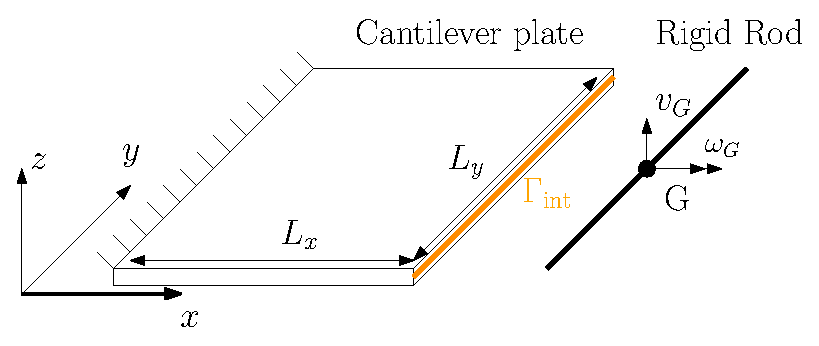
\includegraphics[width=0.9\textwidth]{plate_rod_separated.eps}}
	\only<2>{ 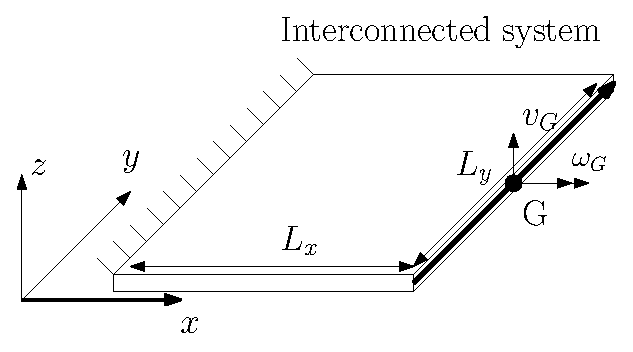
\includegraphics[width=0.7\textwidth]{plate_rod_welded.eps}}
\end{tcolorbox}

\end{frame}

\begin{frame}{Boundary interconnection of the Kirchhoff plate}
The system is composed by a cantilever plate (distributed pH) connected to a rigid rod
\only<1>{
\begin{equation*}
\small \text{dpH} \left\{ 
\begin{aligned}
\diffp{x_1}{t} &= \mathcal{J} \diffd{H_1}{x_1} \\
u_{\partial, 1}  &= \mathcal{B} \diffd{H_1}{x_1} \\
y_{\partial, 1} &= \mathcal{C} \diffd{H_1}{x_1} 
\end{aligned}
\right. \qquad
\text{pH} \left\{ 
\begin{aligned}
\diff{\bm{x}_2}{t} &= {J} \diffp{H_2}{\bm{x}_2} + {B} \bm{u}_2 \\
\bm{y}_{2} &= {B}^T \diffp{H_2}{{x}_2} + {D} \bm{u}_2 \\
\end{aligned}, \qquad 
\right. 
\end{equation*} %

where $u_{\partial, 1}  \in \mathscr{U}, \, y_{\partial, 1} \in  \mathscr{Y} = \mathscr{U}^\prime$ belong to some Hilbert spaces and ${x}_2 \in \mathbb{R}^n, {u}, {y} \in \mathbb{R}^m$. The interconnection is power-preserving if
\[
\left\langle u_{\partial, 1}, \; y_{\partial, 1} \right\rangle_{\mathscr{U} \times \mathscr{Y}} + 
\left\langle {u}_{2}, \; {y}_{2} \right\rangle_{\mathbb{R}^m} = 0.
\]
This is achieved by introducing a compact operator $\mathcal{W}: \mathscr{Y} \rightarrow \mathbb{R}^m$
\begin{equation*}
\label{eq:int_inf}
{u}_2 = -\mathcal{W} \, y_{\partial, 1},  \qquad u_{\partial, 1} = \mathcal{W}^* \, {y}_2,
\end{equation*}
}
	
\only<2>{\vspace{.5cm}\centering 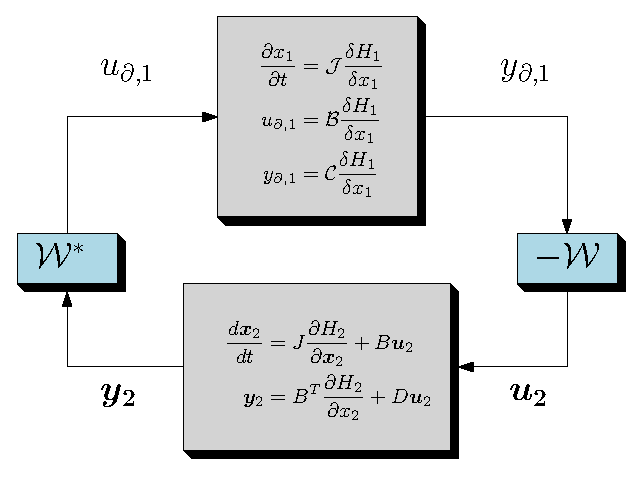
\includegraphics[width=0.6\textwidth]{pp_interconnection.eps}}

\end{frame}

\begin{frame}{Boundary interconnection of the Kirchhoff plate}
\begin{equation*}\small
\begin{aligned}
\text{Plate} \; (\Omega &= [0, L_x] \times [0, L_y]) \\
\begin{bmatrix}
\rho h & 0 \\ 0 & \mathbb{D}^{-1} \\
\end{bmatrix}
\diffp{}{t}
\begin{bmatrix}
\partial_t w \\ \bm{M} \\
\end{bmatrix} &= 
\begin{bmatrix}
0 & -\div\Div \\ \nabla^2 & 0 \\
\end{bmatrix}
\begin{bmatrix}
\partial_t w \\ \bm{M} \\
\end{bmatrix} \\
u_{\partial, \text{pl}} &= \partial_t w (x = L_x, y), \\
y_{\partial, \text{pl}} &= \widetilde{q}_n(x = L_x, y).
\end{aligned} \qquad \quad
\begin{aligned}
\text{Rigid rod} \\
\begin{bmatrix}
M & 0 \\
0   & J_G \\
\end{bmatrix} 
\displaystyle \diff{}{t}
\begin{pmatrix}
v_G \\ \omega_G \\
\end{pmatrix} & = \begin{pmatrix}
F_z \\ T_x \\
\end{pmatrix} = \bm{u}_{\text{rod}}\vspace{1mm}, \\
\bm{y}_{\text{rod}} &= \begin{pmatrix}
v_G \\ \omega_{G} \\
\end{pmatrix},
\end{aligned}
\end{equation*}
Space $\mathscr{Y}$ is the space of square-integrable functions with support on $\Gamma_{\text{int}} = \left\{ (x,y) \vert \; x=L_x, 0 \le y \le L_y  \right\}$.
 The interconnection operator then provides the total force and torque acting on the rigid rod
\begin{equation*}
\mathcal{W} y_{\partial, \text{pl}} =  - \begin{pmatrix}
F_z \\
T_x \\
\end{pmatrix} = \begin{pmatrix}
\int_{\Gamma_{\text{int}}} y_{\partial, \text{pl}} \d{s} \\
\int_{\Gamma_{\text{int}}} \left( y - L_y/2 \right) y_{\partial, \text{pl}} \d{s} \\
\end{pmatrix}.
\end{equation*}
The adjoint operator provides a rigid movement as the plate input at $\Gamma_{\text{int}}$
\begin{align*}
\left\langle \mathcal{W} y_{\partial, \text{pl}}, \; \bm{y}_{\text{rod}} \right\rangle_{\mathbb{R}^m} &= \left\langle y_{\partial, \text{pl}}, \, \mathcal{W}^* \bm{y}_{\text{rod}}\right\rangle_{L^2(\Gamma_{\text{int}})}, \\
\mathcal{W}^* {y}_{\text{rod}} &= v_G + \omega_{G} \left( y - L_y/2 \right).
\end{align*}
\end{frame}

\begin{frame}{Results}
\begin{center}
	\onslide*<1>{
		\setlength{\abovedisplayskip}{0pt}
		\setlength{\belowdisplayskip}{0pt}
		Distributed load ($t_{\text{end}} = 10 \, [\mathrm{ms}]$)
		\begin{equation*}
		p = \begin{cases}
		10^5 \left[ y + 10 \left( y - L_y/2 \right)^2 \right] [Pa], \quad &\forall \, t < 2 \, [\mathrm{ms}], \\
		0, \quad &\forall \, t \ge 2 \, [\mathrm{ms}].
		\end{cases}
		\end{equation*}
		\begin{columns}
			\begin{column}{.45\textwidth}
				\includemedia[
				label=vidNoRod,
				addresource=../../Article_CDC/Videos/Kirchh_NoRod_Slow.mp4,
				activate=pageopen,
				width=6cm, height=5cm,
				flashvars={
					source=../../Article_CDC/Videos/Kirchh_NoRod_Slow.mp4
					&loop=true
				}
				]{}{VPlayer.swf}
			\end{column}
			\begin{column}{.45\textwidth}
				\includemedia[
				label=vidRod,
				addresource=../../Article_CDC/Videos/Kirchh_Rod_Slow.mp4,
				activate=pageopen,
				width=6cm, height=5cm,
				flashvars={
					source=../../Article_CDC/Videos/Kirchh_Rod_Slow.mp4
					&loop=true
				}
				]{}{VPlayer.swf}
			\end{column}
		\end{columns}
	
	\mediabutton[
	mediacommand=vidNoRod:playPause,
	mediacommand=vidRod:playPause
	]{\fbox{Play/Pause}}
				
		%\movie[width=0.8\textwidth, height=0.6\textheight]{Plate and rod}{../Videos/Comparison_RodNoRod.mp4}	
	}
		\onslide*<2>{
			\includegraphics[width=0.48\textwidth]{HamiltonianNoRod_cropped.eps}
			\includegraphics[width=0.48\textwidth]{HamiltonianRod_cropped.eps}
		}
	\end{center}
\end{frame}



\begin{frame}{Conclusion}
The following has been presented:
	
\end{frame}


\begin{frame}{}
\centering
\Huge Thanks for your attention \\
\Huge Questions?
\end{frame}

\begin{frame}[allowframebreaks]{References}
\printbibliography
\nocite{*}
\end{frame}

\end{document}
